\documentclass[11pt, a4paper]{article}

\usepackage[english]{babel}
\usepackage[utf8]{inputenc}
\usepackage{amsmath}
\usepackage{amsfonts}
\usepackage{graphicx}
\usepackage[margin=1in]{geometry}

\usepackage[colorinlistoftodos]{todonotes}

\title{Effects of Uncertainty and Frequency Based Social Learning on Exploration versus Exploitation}

\author{Alina Acosta\footnote{alinaacosta@college.harvard.edu}, Jack Dent\footnote{jdent@college.harvard.edu}, Anna Liu\footnote{annaliu@college.harvard.edu}, Jerry Tang\footnote{jerrytang@college.harvard.edu}}

\date{December 10, 2016}

\begin{document}
\maketitle

\section{Introduction}

Decision-making is a ubiquitous activity shared by individual people, animal populations, and entire societies. Animals search for food, territory, and mating partners. Humans engage in search on a much more complex scale, from choosing which restaurant to go to on a certain day, to whether to do homework or socialize, to which policy proposal to enact to provide the greatest gains to a community. Search in these domains requires balancing a trade-off between pursing what is already known, exploitation, and searching for better opportunities elsewhere, known as exploration. The exploration-exploitation trade-off has been studied by researchers from a diversity of fields, including those exploring how ant colonies find food \cite{Deneubourg1986}, machine-learning theorists in efforts to improve reinforcement learning \cite{Kaelbling} and product placement researchers in franchise stores \cite{Sorenson}.

However, humans usually do not act alone in making decisions. Rather, they incorporate social sources of information with their own to make more optimal choices between exploration and exploitation. For example, customers often resort to Yelp reviews when deciding which dish to pick at a restaurant, or ask classmates about their experiences with different courses before making their course selections for the following semester. However, despite the importance of social information in decision-making, questions still remain as to how individuals integrate different information sources with their prior knowledge. What factors do individuals take into consideration when judging whether to follow their own instincts or group information? How are factors of reliability, time, difficulty of task, and cost to the individual accounted for in search? Several researchers have explored these factors in their models, including Toelch, who discovered that participants employ a "copy-when-uncertain" strategy and deviate from Bayes' optimal when integrating individual with social information \cite{Toelch2013a}. Several of the models in the Toelch paper were borrowed from McElreath \cite{McElreathetalSuccessbias2008}, in which he explores how providing information about payoff and frequency to subjects influenced their decision making. We will build off the McElreath model to further explore how frequency information affects individual choices in the exploration-exploitation trade-off.

Multi-armed bandit problems provide a good model for studying tensions between exploitation and exploration because they offer a direct trade-off between exploring multiple options (trying other arms of the bandit) and exploiting a known source of reward (taking advantage and playing one arm of the bandit). They are inspired by gamblers at rows of slot machines, known as ``one-armed bandits." When played, each bandit arm gives a reward with some probability distribution. The objective is to maximize the sum of rewards after a sequence of playing multi-armed bandit games. 

\section{Ways to Learn Socially}

Given the abundance of information available in any decision an individual makes, we outline the different strategies available below for integrating social  with individual information in multi-armed bandit games.

\subsection{Unbiased Social Learning}
One of the simplest ways to learn socially is to randomly select another individual and copy his or her strategy. This type of behavior is common among children, who have not developed the ability to reason and advanced animals \cite{Wood2013}.

\subsection{Frequency-Dependent Social Learning}
When a large population is available, we can measure how often a particular arm in the bandit is chosen. In positive frequency dependence, the individual copies the most common behavior of the group. This trait is better known as ``conformity", which after several rounds tends to see many individuals grouped around a few specific arms in a multi-armed bandit. 

\subsection{Payoff-Based Social Learning}
In some cases, we are able to observe the payoff that other players get from choosing certain arms. Payoff based learning is reliable, since the payoff that everyone sees is objective. Even if the frequency of people choosing option one option is low, if the payoff of that option is high, then the option may be a better choice than the other arms.

\subsection{Copy-when-uncertain}
Individuals often use social information when uncertain about their own information in a stock-market game \cite{Toelch2013a}. If given the choice to invest in different options, individuals will copy others' strategy, but they will be cautious about investing when copying. Often times, your own information may not be as reliable as the group information, which results in a copy-when-uncertain strategy.

Conformity to majority opinions increase when solutions to math problems were not clear \cite{Laughlin_1986}, and other researchers discovered that conformity increases with more difficult perceptual tasks \cite{Baron_1996}.

\subsection{Integrated social learning}
There are numerous ways to mix the above strategies. Due to individual differences in personality, age, skill, and current environment, some strategies will be more common among certain individuals than others. Individuals who are more egocentric may weigh their own information higher even when uncertain. Sometimes, payoff information is not available or delayed, forcing individuals to resort to one of the other strategies.

\section{Motivation}

Our motivation for this project built off of our project on exploration versus exploitation with no social parameters. Cohen \cite{Cohen2007} introduces a variety of information about current research on exploitation versus exploration. Cohen discusses how acetylcholine and norephinephrine are used to signal expected and unexpected uncertainty, which is likely to influence the decision to explore or exploit. The paper explains how norepinephrine in the locus coeruleus has two distinct modes: ``tonic mode" and ``phasic mode". Tonic model favors exploration and phasic mode favors exploitation. Cohen also introduces the way the dopaminergic system could implement reinforcement learning mechanisms that could be used in the decision to exploit or explore. In the Cohen paper, social signals are also mentioned as an important factor in deciding to exploit or explore, which is the initial inspiration behind our current topic. 

The behavioral data with regard to social influence on exploration versus exploitation also exemplifies the power social influence can have on an individual. For example, one study examined how social influence can undermine the wisdom of crowd effect \cite{Lorenz2011}. It has been shown that median estimates of a group can be more accurate than estimates of experts. In this experiment, they allowed subjects to adjust their answer to a factual question after being given either the median estimate or the full information of estimates of the group. This knowledge caused estimates to narrow significantly compared to subjects that were not given social information. This caused the crowd to become less reliable and the wisdom of crowd effect was lost \cite{Lorenz2011}. We took both this empirical data and behavioral data to construct a model by which an individual's information is weighted with group information, where the weights are determined by uncertainty and an individual's egocentrism. 

\subsection{Model Motivation} 
A few more recent papers acted as the inspiration for what we hoped our model would accomplish. Toelch et al. \cite{Toelch2013a} examined the conditions under which individuals changed their decisions after incorporating social information, finding that they tended to be consistent in their propensity to use and value social information \cite{Toelch2013a}. Another study done by Toelch looked at optimal exploitation of social information under uncertainty \cite{Toelch2013} and, as mentioned above, found that individuals tended to deviate from Bayes optimal choice when integrating individual information with social information. Both of these were items which we considered important to incorporate into our model.

We had several objections to many of the models we found in existing literature review. Firstly, payoff information is often unavailable to individuals because the other agents do not make their payoffs known. The McElreath paper \cite{McElreathetalSuccessbias2008} proposed a model that incorporated frequency and payoff information to fit their observations that participants used a hierarchical strategy that primarily uses payoff information, but in most cases, we dispute that payoff information will be available. Secondly,  in the McElreath model, frequency information is linearly added to individual's payoff information, but we see these two types of information as inherently different, and argue that they should not be combined linearly. Thirdly, many models do not account for individual compared to group certainty, which as Toelch \cite{Toelch2013} describes is a crucial factor for determining how heavily to weigh individual versus group information.

\subsection{Neural Correlates Motivation}
As introduced above, there are many suggested pathways that affect exploitation versus exploration. Jepma et al. \cite{Jepma_2011} used pupil diameter as a proxy for locus coeruleus-norepinephrine (LC-NE) levels. There are two key findings in this paper that are relevant to our research. Firstly, the paper found that exploratory choices were preceded by larger baseline pupil diameters than exploitative choices. Secondly, the paper found that individual differences in baseline pupil diameter were good predictors of an individual's tendency to explore. However, we were also inspired by Frank et al. \cite{Frank2009}. In Frank's research they found two genes controlling striatal dopamine function, DARPP-32 and DRD2, were associated with exploitative learning to adjust response times as a function of positive and negative decision outcomes. They also found the Catechol-O-methyltransferase (COMT) gene, which controls prefrontal dopamine function, is associated with 'directed exploration' and this function varies between individuals. Individuals with the Met/Met allele were more likely to use an ``uncertainty bonus" when making decisions. 

In our paper, we decided to examine dopamine over the LC-NE system for two main reasons. Although pupil diameter is an easy and noninvasive way of potentially studying LC activity, the correlation has not been rigorously proven to be true. There are preliminary data but we would like to find something more rigorous to examine. Second, there is existing data relating dopamine to behaviors of conformity. Although conformity is different than social influence on the decision to explore or exploit, it can be expected that individuals who are more likely to conform are also more easily influenced by the decisions of others. We will use this as the basis of our predictions knowing that it is possible that it is possible empirical data may show something different.

Specifically, we would like to look at dopamine D2 receptor in the striatum. Frank et al.\cite{Frank2009} explained that the DRD2 gene is associated with the density of D2 receptors in the striatum. People with that are T/T carriers are shown to increased D2 receptor densities. Those with at least one C allele had show lower D2 receptor concentrations. Additionally, they found that stimulating dopamine receptors caused faster reaction times when a faster reaction time had increased expected value but impeded the ability for an individual to slow down their reaction time when a slower reaction time increased expected value. Relatedly, they discovered that dopamine depletion caused individuals to improve at slowing down their reaction time, when a slower reaction time produced a higher expected value. It has also been shown that D2 receptor binding potential is inversely related to social conformity \cite{Sigray2014}. Our approach hopes to integrate these three findings to answer the question: ``how do innate dopamine receptor densities affect an individual's propensity to favor social information in the context of exploration versus exploitation?"

\section{Social Learning for Multi-Armed Bandits}

Our model shows how social information can be used to enhance performance in a certain formulation of the $K$-armed bandit problem. In our model, the player combines two sources of information to determine their posterior belief for the payoff distributions of each arm. In addition to their own priors for the payoff distribution from the previous round, the player also gets to observe the decisions of the other players at each round, which potentially gives them valuable information about the payoff distributions for each arm.

The actual observed variable for social information, in our model, is the number of players that chose each arm. Intuitively, the expected payoff for each arm should increase in line with the number of the players that choose that arm. Additionally, the distribution of the group's choices across the arms will affect the informational value of the social signal. For example, if the group has overwhelmingly chosen a single arm, the player has reason to believe that arm has a high payoff under the assumption that other players are also looking maximize their rewards. On the other hand, if the group choices are uniformly distributed across the arms, the player does not obtain much in the way of social information to motivate her own choice. It is important to note that the player does not get to observe the actual payoffs that other players received from their choices of arm.

An example of using frequency as a proxy for potential payoff is excitement about a new restaurant. An individual may know which restaurants they like in their neighborhood with high certainty. Now, imagine that a new restaurant comes to town. The individual continuously hears about how good this restaurant is from friends and is eventually convinced to try eating there. Even though the individual could not see the payoffs that his friends received from eating at this restaurant, the sheer number of people who have praised this restaurant is enough of a signal for the individual to switch from choosing between his usual restaurants to trying this new one. 

Our model will also show how social information can modulate the balance between exploration and exploitation to improve individual player behavior. As the player becomes more certain in her own predictions, she may choose to explore the arms less, preferring to exploit her prior information about payoff distributions. However, if the player observes that the group predictions consistently outperform her own, she may choose to give more weight to group predictions than her own when making future choices. Since social information and individual information will differ at least slightly in some cases, our model will show that the balance between individual and social information can provide valuable additional information about when an individual player should ``explore" more. In this case, ``exploration" does not mean randomization, but a choice of how much of the group predictions to factor into decisions. In contrast, which we define exploitation as the greedy policy of always selecting the optimal action given your individual information. When exploring, social information may cause you to completely disregard your own judgments in favor of a different heuristic. 

\section{Experimental Setup}
In order to study frequency dependence in a multi-armed bandit, we modified the farming game proposed in McElreath. In this game, a large group of participants each make decisions to plant and receive yields from crops over a set number of seasons. Each season represents a decision to plant and receive a yield from a certain type of crop. Which crop the participants chose represent the arm of the \textit{K}-armed bandit. 

After the first round, participants can access social information from the most recent period. Participants could examine the number of other individuals who chose each type of crop. In this sense, they could see how frequently each type of crop was being chosen by the other participants in the experiment.

\begin{figure}[h]
\centering
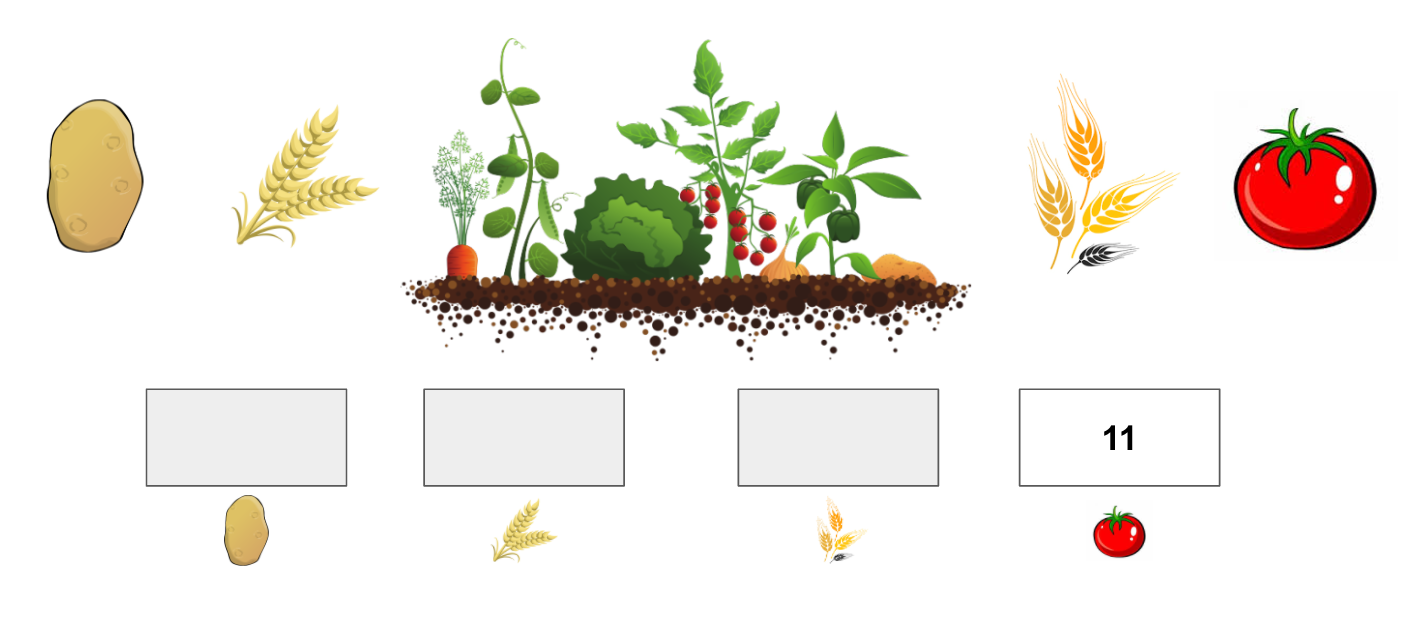
\includegraphics[scale=0.4]{farm.png}
\caption{Farm game setup, in which players can choose one of the crops shown in each season. They can hover over the gray boxes at the bottom of the screen to see how many other participants picked a particular crop in the past round.}
\end{figure}

To explore the neural correlates of this experiment a few selected participants would play the game while being examined using positron emission tomography (PET) and a radioligand to show D2 receptor potential values. Participants in the scanner would be selected based on their DRD2 genotype. There would be a group of T/T carriers and then a group of people that have at least one C allele since this is what was used in the Frank et al. paper to distinguish between those with high D2 receptor densities and those with a lower concentration of D2 receptors. 

\section{Integrated Uncertainty Model}

We will now outline our proposed model to solve the multi-armed bandit exploration-exploitation problem with integrated social information. Both the exploration-exploitation process and the social learning process are driven by uncertainty, and our model hopes to integrate these two effects of uncertainty in explaining our choices. At each opportunity to choose an arm, our player decides which action to take in three separate steps.

\begin{enumerate}
\item Firstly, the player combines two sources of information to predict the expected reward payoffs for each arm. The player calculates an estimate for the value that the group attributes to each arm from the distribution of the group members across the different choices. She then combines this estimate with her own prior for the distribution of payoffs for each arm. Put together, the two information sources allow the player to improve her prediction accuracy by harnessing both her individual beliefs and the power of social information.
\item Secondly, the player chooses an arm to visit based on her calculations for the expected payoffs. In this step, the player could potentially also use social information to determine the amount of exploration. For the purposes of our model, however, the rate of exploration is determined only by the accuracy of past predictions, and is not informed by group activity other than the impact that group information has on prediction in the first step.
\item Finally, the player visits her choice of arm, samples a reward, and updates her prior reward distribution for the next round with the observed reward value.
\end{enumerate}

\subsection{First step: predict expected rewards}

The true reward distribution from arm $i$ of the bandit is given by the Gaussian distribution $A_i \sim \mathcal{N} (\alpha_i, \beta_i^2)$, so the player's prediction for the payoff distribution parameters is the conjugate prior for the payoff distribution. At round $n$, the player estimates that arm $i$ has distribution $S_i(n) \sim \mathcal{N} (\mu_i(n), \sigma_i(n)^2)$. Initially, we set $S_i(n) \sim \mathcal{N} (\mu(0), \sigma(0)^2) \forall i \in [1, k]$. Likewise, the payoff distribution derived from the social information for each arm $i$ at round $n$ is given by $G_i(n) \sim \mathcal{N} (\rho_i(n), \lambda_i(n)^2)$.

\subsubsection{Calculating expected payoff from group frequencies}

We use maximum likelihood estimation to calculate the most likely parameter value $\rho(n)$, where $\rho_i(n)$ is the payoff for each $G_i(n)$. Formally, $\hat{x}(n)$ represents vector of arm choices $i$ where $i \in [1, k]$ for each player. $\hat{x}(n) \in [1, k]^m$, and we find the parameter values for a Gaussian distribution that maximizes the chance of observing $\hat{x}(n)$. Note that our likelihood estimation for $\rho(n)$ depends on the entire vector $\hat{x}(n)$, not just on the count $\hat{x}_i(n)$, since the distribution of the group's choices across all arms will affect our estimate for group's payoff prediction for a single arm.

Thus, Bayes' Rule gives

$$P(\rho(n)|\hat{x}(n)) \propto P(\hat{x}(n)|\rho(n))P(\rho(n))$$.

To calculate the conditional probability of obtaining the group choice vector $\hat{x}(n)$ given $\rho(n)$, we observe that

\begin{align*}
P(\hat{x}(n)|\rho(n)) & = \prod_{i=1}^m P(\hat{x}_i(n)|\rho(n)) \\
& = \prod_{i=1}^m \frac{\exp(\beta \cdot \rho_{\hat{x}_i}(n))}{\sum_{j=1}^k \exp(\beta \cdot \rho_j(n))}
\end{align*}

where $m$ is the number of agents making choices regarding which arm to pick and $\beta$ is a parameter chosen to best fit our results.

Finally, having determined the distribution $P(\rho(n)|\hat{x}(n))$ of parameter values, we can calculate the conditional expected value of the parameters $\rho(n)$, given $\hat{x}(n)$. We have now fully specified the group reward payoff estimate, give by $G_i(n) \sim \mathcal{N} (\mathrm{E}[\rho_i(n)|\hat{x}], \lambda_i(n)^2)$.

\subsubsection{Combining Individual and Group Signals}

Alais and Burr have suggested that we can optimally combine multimodal information sources by summing the individual and group signals with certain weights \cite{Alais_2004}. For each arm, we want to weigh our own payoff prediction given by our priors against the inferred payoff prediction given by the group frequencies. Four factors go into this weight: the actor's uncertainty in the given arm, the group's uncertainty across all arms, the level of trust in the group for the given arm, and the actor's innate egocentrism parameter. Thus, the weighted expected payoff at time $n$ is given by the equation 

$$R_i(n) = \epsilon v_i(n)w_i(n) \times S_i(n) + (1 - \epsilon v_i(n)w_i(n)) \times G_{i}(n|\hat{x}(n))$$

$\epsilon$ represents egocentrism, which varies across individuals and represents how much an individual would trust their own information compared to group information prior to receiving any data. Considerable individual differences exist in propensity to use social information, as shown by previous studies \cite{EFFERSON_2008}

The variance weight $v_i(n)$ is given by $\frac{\sigma_{g}(n)^2}{\sigma_{i}(n)^2 + \sigma_{g}(n)^2}$, where $\sigma_{g}(n)^2$ is the group variance and $\sigma_{i}(n)^2$ is the actor's variance for arm $i$. 

$w_i(n)$ is our trust parameter for arm $i$, which is updated according to the difference in prediction errors between the actor and the group. For the model to be optimal in the variance-minimization sense, $w_i(n)$ should always be 0.5. In many situations, however, players have been shown to diverge heavily from optimal behaviour. Toelch (2013) has shown that individuals systematically deviate from Bayes optimal when integrating individual with social information, weighing individual information heavily and scales with the accuracy of individual information. When $w_i(n)$ is very large, the player only factors in her prior, which may occur in situations where the individual is very certain in her estimates. When $w_i(n)$ is very small, however, the player relies most heavily on the social information signal, which could occur when in situations when the user has very little prior knowledge. We can model this through the following equation:

$$w_i(n+1) = \frac{\delta_s(n)}{\delta_g(n) + \delta_s(n)}$$

If the individual received a reward $r(n)$ from arm $i$ at round $n$, then the prediction error from the individual's signal is given by $\delta_s(n) = \left|r(n) - \mathrm{Var}[S_i(n)]\right|$. On the other hand, the prediction error from the group signal is given by $\delta_g(n) = \left|r(n) - \mathrm{Var}[G_i(n)]\right|$.

When $\delta_s(n)$ dominates $\delta_g(n)$, $w$ will be close to 1, and the individual will favour their own prediction over the social signal. When $\delta_g(n)$ dominates $\delta_s(n)$, $w_i(n+1)$ will be close to 0, and the individual will weight the group signal much more heavily.

\subsection{Second step: choice of action}

As stated above, we chose not to integrate social information directly into our own beliefs about the expected payoffs of each arm after calculating the expected rewards. Instead, we rely on the parameter $w_i(n)$ to modulate the extent to which the individual values the group signal.

Given our weighted array of expected payoff means, we run the array through a softmax function to get an array of probabilities for choosing each arm. The actor then chooses an arm to act upon based on these probabilities.

\subsection{Third step: obtain sample and update prior}

After choosing an arm, $R_i(n) \in (R_1(n), \ldots, R_k(n))$ in round $n$, we sample a value from that arm, and receive a reward $r(n)$. For all other arms $j \neq i$, the individual prior distribution for round $n+1$ is directly given by the reward distribution since the sample from arm $i$ provides no new information about their reward distributions. For arm $i$, however, we should update our reward distribution by taking into account the sample reward. Thus the individual prior distributions for round $n+1$ are given by the function.

$$
S_j(n+1) = 
\begin{cases}
R'_i(n)	    & \text{if } i = j \\
R_j(n)      & \text{otherwise}
\end{cases}
$$

To calculate $R'_i(n)$, we note that for each arm, we model the conjugate prior for our estimate of the mean. By the Gaussian conjugacy, for a prior with hyperparameter $\mu_0, \sigma_0^2$, the posterior hyperparameters are $$\mu_1 = \frac{\frac{\mu_0}{\sigma_0^2} + \frac{r_i}{\sigma^2}}{\frac{1}{\sigma_0^2} + \frac{1}{\sigma^2}}, \sigma_1^2 = (\frac{1}{\sigma_0^2} + \frac{1}{\sigma^2})^{-1}$$ on observing the single reward $r_i$, where $\sigma^2$ is the known variance of the underlying distribution. If we wish to drop the assumption that the variance of the arms are known, the estimates for the mean and variance of each arm can be modeled using a normal-inverse gamma conjugate prior.

\section{Simulations}

To understand how our model would work in practice, we simulated the farming problem with five crops, 160 rounds, and a group of 120 other farmers. The payoff for each crop is represented as a normal distribution with $\sigma^2 = 1$ and means drawn from an underlying $\mathcal{N}(5, 2)$ distribution. This gave us a crop payoff distribution vector $$[\mathcal{N}(3, 1), \mathcal{N}(5, 1), \mathcal{N}(6, 1), \mathcal{N}(7, 1), \mathcal{N}(8, 1)]$$ The actor models the mean payoff of each crop using a normal distribution, which is updated in a Bayesian inference process at the end of each round following observation of the actual reward. Following the model described above, at each step the actor creates a payoff vector using her prior for the distribution means, and then infers the payoffs from the group frequency vector using a maximum likelihood estimate. She then weighs these two predicted payoff vectors using her uncertainty, the group's uncertainty, the error weight, and the $\epsilon$ parameter representing her individual egocentrism. A softmax function is then applied to this weighted payoff prediction vector to obtain probabilities for choosing each arm. On selecting an arm, the actor updates her priors given the observed reward. 

To see how the model performs under different circumstances, the two variables we focus on are the group frequency patterns and the personal egocentrism constant $\epsilon$. For the group frequency patterns, we create two different frequency profiles, a ``good" group with a frequency proportional to the payoffs and a ``bad" group that is evenly distributed across the 5 crops. Formally, the good group had a frequency profile $(12, 20, 25, 29, 33)$, while the bad group had a frequency profile $(24, 24, 24, 24, 24)$. This is driven by our desire to see how our social learning model moves from exploration towards exploitation based on what the group is choosing. We also vary our epsilon parameter between a high epsilon level $\epsilon = 0.9$ and a low epsilon level $\epsilon = 0.4$ corresponding to high and low levels of personal egocentrism, reflecting our desire to model how different individuals may have different responses to group information. 

Finally, we made a few assumptions about the payoff distributions for each crop in order to fit our social-based exploration-exploitation model into the farming problem. For the sake of simplicity and to isolate our variables of interest, we assume that the crops have an equal variance which is known to the user. We also assume that the crop rewards are drawn from some underlying distribution, which is known to the user as well; this
prior over different payoff means normalizes the Bayesian process of predicting payoff profiles from group frequency patterns. This is a valid assumption because while the farmers don't know how certain crops may perform, they have a prior understanding of how crops should perform in general.  

Running the simulation using our four possible variations (low $\epsilon$ bad group, high $\epsilon$ bad group, high $\epsilon$ good group, low $\epsilon$ good group), we obtained the following results, which were largely consistent with the intuition of how our model should have performed.

\begin{figure}[h]
\centerline{%
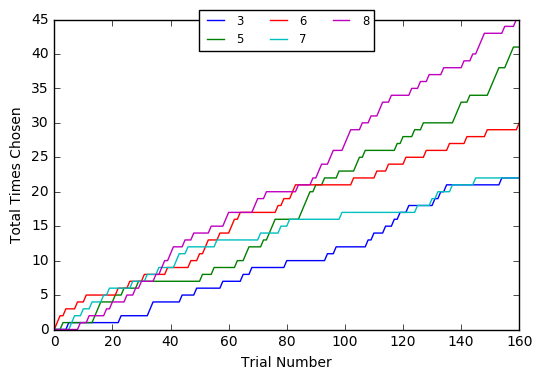
\includegraphics[width=0.5\textwidth]{low_beta_bad_group}%
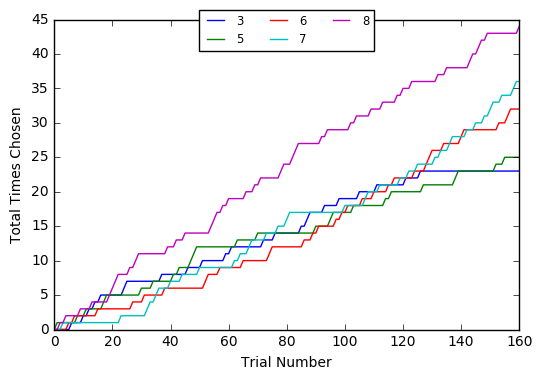
\includegraphics[width=0.5\textwidth]{high_beta_bad_group}%
}%
\centerline{%
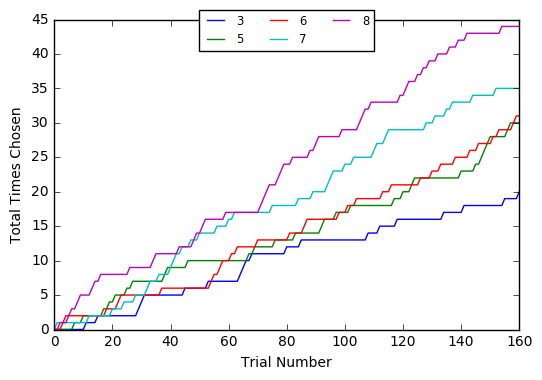
\includegraphics[width=0.5\textwidth] {high_beta_good_group}%
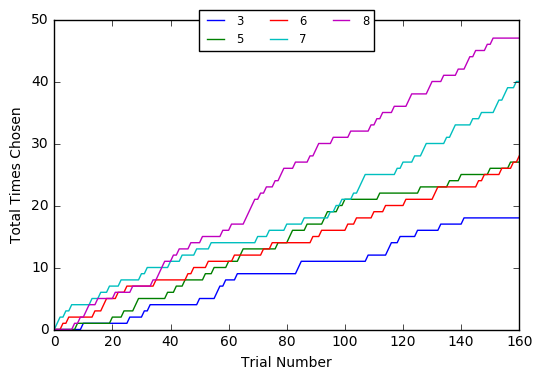
\includegraphics[width=0.5\textwidth] {low_beta_good_grou}%
}%
\caption{Simulations: Clockwise from top left: low $\epsilon$ bad group, high $\epsilon$ bad group, low $\epsilon$ good group, high $\epsilon$ good group. The number corresponding to each line represents that arm's mean payoff}
\end{figure}

\begin{itemize}
	\item Low $\epsilon$, bad group: while the best crop won out, you can see it was closely followed by the crops with payoffs 5 and 6, with the second best crop rarely chosen. This is what we would expect from actors with low egocentrism following an evenly distributed group: one is inclined to utilize the group information at each step, but the group information suggests that the underlying payoffs are very similar and around average. This causes the user to choose almost randomly, explaining the result that the times chosen are fairly uncorrelated with the actual payoffs.

	\item High $\epsilon$, bad group: in contrast, if the actor is egocentric, she discounts how the group performs in favor of her own experiences. We see that our best option differentiates itself, while the other options eventually finish in the expected order. However, it is clear that it takes a while before the actor starts exploiting: only around the 120th trial do the low reward crops start tapering off. This is in line with the idea that with little group help, the egocentric actor must explore more to decide which crops are the best.

	\item High $\epsilon$, good group: we see similar results as we did in the high $\epsilon$ bad group case, which is intuitive since a change in the group performance doesn't strongly affect egocentric actors. Once again we get that the bad results taper off near the end, the good results dominate but don't distinguish themselves until halfway through the process. This actor does perform better, as the group's success in predicting rewards raises the group trust weight, which balances out the egocentrism parameter to raise the group weight relative to the previous experiment.

	\item Low $\epsilon$, good group: in the final experiment, note that the amount of exploitation occurs earlier than it does in the other ones; the low $\epsilon$ actor takes advantage of the (helpful) group effect to learn which options are good without having to explore as much herself, allowing her to be confident enough to exploit the best option earlier in the process (around trial 60). 
\end{itemize}

\section{Neural Correlates}
The egocentrism parameter is a key feature of our model. Not all people make decisions the same way and this is a key way of distinguishing that. Knowing that D2 receptor bind potential in the striatum is inversely related to social conformity \cite{Sigray2014}, we can make predictions about an individual's egocentrism parameter. A person that is a T/T carrier for the DRD2 gene is known to have a high density D2 receptor density \cite{Frank2009}. Therefore it is expected that a person that is a T/T carrier would be less likely to conform. In terms of social influence on exploration versus exploitation, this would imply an individual would be less likely to value the information provided by the group, more likely to exploit their own information and have a higher egocentrism parameter. This can be seen in the simulations above when there it is run with a large $\epsilon$ value. In both cases of accurate information from the group or inaccurate information from the group, the decision making process remains fairly similar and eventually the correct order is determined. Similarly, a person that has at least one C allele would have a lower D2 receptor density and therefore be more likely to conform. In this case we would expect an individual to favor the group's information over their own and have a lower egocentrism parameter. The simulations for this can also be seen above in examples with a low $\epsilon$ value. When the subject is given inaccurate information, they utilize this information but therefore do not appropriately pick the crops that will give them the highest payoff. When the subject is given correct information they determine the appropriate payoffs and exploit them more quickly due to their utlilization of social information.

More broadly, we could expand this experiment to examine the effects of over stimulation of dopamine receptors and dopamine depletion. This was similarly done by Frank et al. \cite{Frank2009} to examine the effects on reaction time in decision making. In the Frank paper they found that over stimulation of dopamine receptors caused faster reaction times for experiments in which a faster reaction time was preferred, but impeded the ability to slow down for experiements where a slow reaction time was preferred. This is compared to normal participants in which a decreasing reaction time and increasing reaction time were not related. Since the D2 receptor was shown to have been associated with slowing down reaction rates \cite{Frank2009}, this result suggests that the effect of the D2 receptor basically becomes nonexistent. If we were to stimulate dopamine receptors in our experiment we would expect to see a significant decrease in the egocentrism parameter so to increase the value of social information. We also saw in the Frank paper that a depletion in dopamine led to better ability to slow down reaction time and difficulty increasing reaction time. The exact opposite result of stimulation. Examining the brains of participants with Parkinson's would also be an ideal way of looking at the way in which a dopamine depletion would affect an individual's preference for social information. We can predict that depleting dopamine would have the opposite effect of stimulation, meaning the individual would have a much higher egocentrism parameter. If we were to see results significantly different than those predicted here, it would give new insights into if and how conformity and social influence pathways differ within the brain.

\section{Discussion}
Throughout the decision making process, an individual often has to choose between exploiting an existing known option or exploring a new option. This decision making process has been examined mainly in isolation. However, our lives consist of constant interactions. It is unrealistic to make a model that looks solely at making decisions in isolation. The question we posed was, ``How does knowing the choices of others affect an individual's decision to explore or exploit?" A key difference in our research is that we did not want the individual to know the payoffs of another person's decision: we simply examined frequency of group choices since often in real life you can only see people making decisions and do not know what the outcomes of those decisions were.

Our inspiration for how to pursue answering this question began with Toelch \cite{Toelch2013}. Toelch's paper was part of series of two works that looked at how social influence affects one's decision to explore or exploit. Both of which provided key information in the production of our model. We were similarly inspired by behavioral data that suggests individuals conform somewhat easily when they are uncertain about their own information \cite{Lorenz2011}, and neural data that uses dopamine as a way of examining an individual's decision to explore or exploit. We designed an experiment where subjects make decisions about what crops to plant and receive yields from crops over a series of seasons. Participants are able to access social information from the past season to examine the number of individuals that selected a certain crop. This is a way of measuring how the frequency of others' decisions affects an individual's decisions. To explore the neural correlates, participants would be selected to play the game while being examined using PET and a radioligand to show D2 receptor potential values. Subjects would be selected for the scanner based on their genotype, since the DRD2 gene is associated with D2 receptor densities in the striatum \cite{Frank2009} and D2 receptor densities are inversely related to social conformity \cite{Lorenz2011}.

Our model aims to combine an individual's knowledge with the information attained from the group. The model also accounts for individual uncertainty versus group uncertainty as well as a constant to represent an individual's tendency to favor their own information over the group's information: our egocentrism parameter, $\epsilon$. 

The purpose of the PET scan is to examine how D2 receptor densities affect an individual's decision to value social information. We hypothesize that an individual with a higher D2 receptor density will be less likely to value social information and there for have a large egocentrism parameter. The effects of different egocentrism parameters can be seen in our simulations and accurately reflect the expected behavior of individuals that vary in how they value social information, whether that information is correct or not. 

In future work, we would want to explore how the composition of the group affects our trust in the group, for example, between family members and strangers. We would also like to explore alternative options to estimate payoffs from frequencies, and explore different routes of integrating frequency information into our decision-making process. Understanding how different factors influence our decision-making processes will be crucial to gaining insights into other human behaviors, such as groupthink, compulsiveness, inattentiveness, and dominance.

\newpage

\nocite{*}
\bibliographystyle{plain}
\bibliography{cited.bib}

\end{document}